%Information relative au document
% !TEX encoding = MacOSRoman
\documentclass[a4paper,12pt]{report}

%Paquets
\usepackage[applemac]{inputenc}
\usepackage[T1]{fontenc}
\usepackage{lmodern,textcomp}
\usepackage[frenchb]{babel}
\usepackage{textcomp}
\usepackage{graphicx}
\usepackage{amsmath}


%D�but du rapport
\begin{document}

%Page de garde
\title{Rapport n�1 MT12}
\author{Alexandre Ballet et Simon LAURENT}
\date{Printemps 2016}
   
  %  \begin{minipage}{0.4\textwidth}
     % \begin{flushleft} \large
        %\emph{Enseignant :} M. Dajlil Kateb\\
        %\emph{Etablissement : } Universit� de Technologie de Compi�gne
      %\end{flushright}
    %\end{minipage}
\maketitle

%Table des mati�res
\tableofcontents

%Exercice 1
\chapter{S�rie de Fourier}

%Exercice 2
\chapter{Classe de fonctions}
	\begin{enumerate}
	\item $f(x)=(sin\,x)^{1/3}$ \\ \\
	La fonction f est d�finie sur l'intervalle ($-\pi;\pi$). Elle est compos\'ee d'une fonction sinus, ce qui la rend impaire. Elle n'admet aucune valeur interdite et on a $f(0^+)=f(0^-)=\sqrt{0}=0$. Elle est donc continue.
	\begin{figure}[ht]
		\centering
		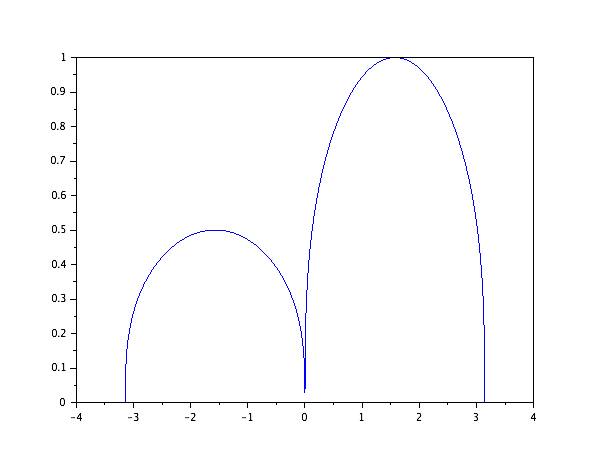
\includegraphics[scale=0.6]{ex2_fig1.png}
		\caption{\label{figure1}Courbe de la fonction $f$.}
		\end{figure}
		\\
	Sa d\'eriv\'ee est $f'(x)=\frac{1}{3} cos x (sin\,x)^{-2/3}$. Elle admet une asymptote verticale en $0$ et n'est donc pas continue.
	La fonction $f$ est continue mais non d\'erivable sur ($-\pi;\pi$).\\ \\
	% Faut-il ajouter le programme Scilab ? Que veux dire "Commenter" ?
	\item $f(x)=(sin\,x)^{4/3}$ \\ \\
	La fonction f est d�finie sur l'intervalle ($-\pi;\pi$). Elle n'admet aucune valeur interdite et on a $f(0^+)=f(0^-)=\sqrt[3]{0}=0$. Elle est donc continue.
	\begin{figure}[ht]
		\centering
		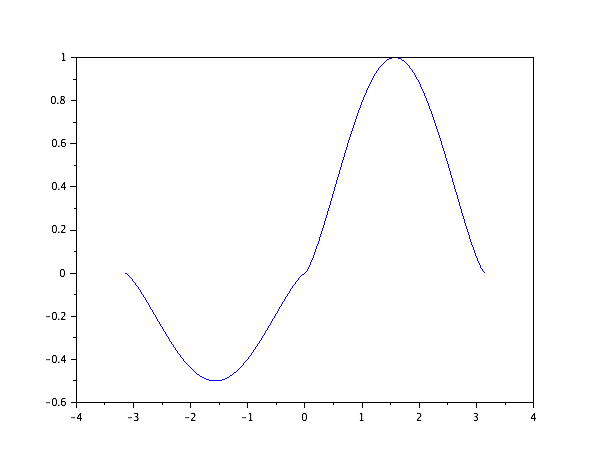
\includegraphics[scale=0.6]{ex2_fig2.png}
		\caption{\label{figure2}Courbe de la fonction $f$.}
		\end{figure}
		\\
	Sa d\'eriv\'ee est $f'(x)=\frac{4}{3} cos\,x (sin\,x)^{1/3}$. Elle n'admet pas d'asymptote et est donc continue.
	La fonction $f$ est continue et d\'erivable, donc r\'eguli\`ere.\\ \\
	\item $f(x)=
  \left\{
      \begin{aligned}
        cos\,x\quad , si\quad x > 0\\
        -cos\,x\quad ,si\quad x \le 0\\
      \end{aligned}
    \right.$ \\
	La fonction f est d�finie sur l'intervalle ($-\pi;\pi$). Elle n'admet aucune valeur interdite et on a $f(0^+)=1$ et $f(0^-)=-1$. Elle n'est donc pas continue en 0.
	\begin{figure}[ht]
		\centering
		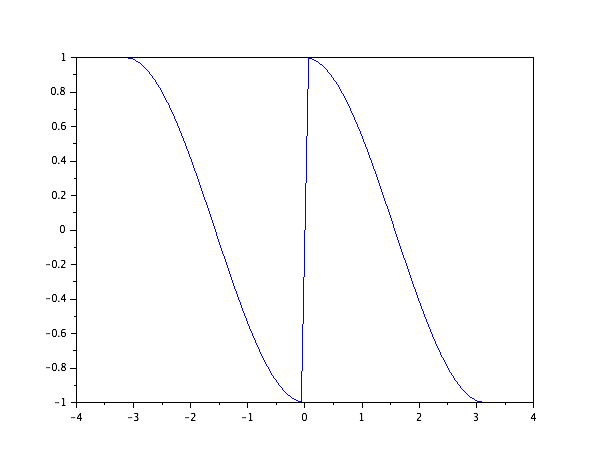
\includegraphics[scale=0.6]{ex2_fig3.png}
		\caption{\label{figure3}Courbe de la fonction $f$.}
		\end{figure}
		\\
	Elle est d\'erivable par morceaux et sa d\'eriv\'ee est $f'(x)=
  \left\{
      \begin{aligned}
        -sin\,x\quad , si\quad x > 0\\
        sin\,x\quad ,si\quad x \le 0\\
      \end{aligned}
    \right.$ \\
	La fonction $f$ est continue par morceaux et d\'erivable par morceaux, donc r\'eguli\`ere par morceaux.\\ \\
	\item $f(x)=
  \left\{
      \begin{aligned}
        sin\,x\quad , si\quad x > 0\\
        -sin\,2x\quad ,si\quad x \le 0\\
      \end{aligned}
    \right.$ \\ \\
	La fonction f est d�finie sur l'intervalle ($-\pi;\pi$). Elle n'admet aucune valeur interdite et on a $f(0^+)=f(0^-)=0$. Elle est donc continue.
	\begin{figure}[ht]
		\centering
		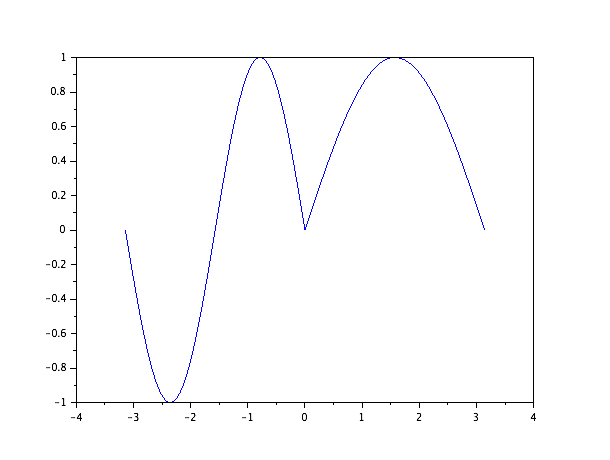
\includegraphics[scale=0.6]{ex2_fig4.png}
		\caption{\label{figure4}Courbe de la fonction $f$.}
		\end{figure}
		\\
	Elle est d\'erivable par morceaux et sa d\'eriv\'ee est $f'(x)=
  \left\{
      \begin{aligned}
        cos\,x\quad , si\quad x > 0\\
        -2cos\,2x\quad ,si\quad x \le 0\\
      \end{aligned}
    \right.$ \\
	La fonction $f$ est continue et d\'erivable par morceaux, donc r\'eguli\`ere par morceaux.\\ \\
	\item $f(x)=
  \left\{
      \begin{aligned}
        (sin\,x)^{1/5}\quad , si\quad x < \pi/2\\
        -cos\,x\quad ,si\quad x \ge \pi/2\\
      \end{aligned}
    \right.$ \\ \\
	La fonction f est d�finie sur l'intervalle ($-\pi;\pi$). Elle n'admet aucune valeur interdite et on a $f(0^+)=f(0^-)=\sqrt{0}=0$ et $f(\pi/2)=0$ et $\lim\limits_{\substack{x \rightarrow \pi/2 \\ x>\pi/2}} f(x)$. Elle est continue en 0 mais pas en $\pi/2$, elle est donc continue par morceaux.
	\begin{figure}[ht]
		\centering
		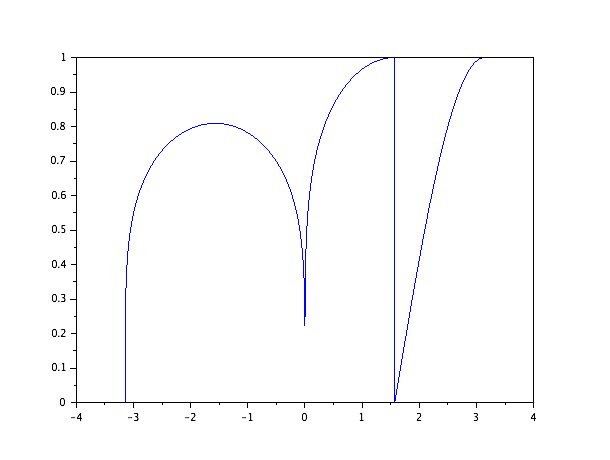
\includegraphics[scale=0.6]{ex2_fig5.png}
		\caption{\label{figure5}Courbe de la fonction $f$.}
		\end{figure}
		\\
	Elle est d\'erivable par morceaux et sa d\'eriv\'ee est $f'(x)=
  \left\{
      \begin{aligned}
        \frac{1}{5}cos\,x\,(sin\,x)^{1/5}\quad , si\quad x < \pi/2\\
        sin\,x\quad ,si\quad x \ge \pi/2\\
      \end{aligned}
    \right.$ \\
	La fonction $f$ est continue par morceaux et d\'erivable par morceaux, donc r\'eguli\`ere par morceaux.\\ \\
	\end{enumerate}
%Exercice 3
\chapter{Ph�nom�ne de Gibbs}

%Exercice 4
\chapter{Application des s�rie de Fourier}
\section{La corde pinc�}
\section{La corde frapp�e}

%Exercice 5
\chapter{Equation de la chaleur}

%Compl�ment au TP
\chapter{Compl�ments}
\section{Finance}
\section{Informatique}

%Test de texte
Comme le disait Jean de la Fontaine dans sa fable :
\begin{quote}
Rien de sert de courir, il faut partir � point.
\end{quote}


\end{document}